% Copyright (c) 2022 Alexander Bluhm <bluhm@openbsd.org>
%
% Permission to use, copy, modify, and distribute this software for any
% purpose with or without fee is hereby granted, provided that the above
% copyright notice and this permission notice appear in all copies.
%
% THE SOFTWARE IS PROVIDED "AS IS" AND THE AUTHOR DISCLAIMS ALL WARRANTIES
% WITH REGARD TO THIS SOFTWARE INCLUDING ALL IMPLIED WARRANTIES OF
% MERCHANTABILITY AND FITNESS. IN NO EVENT SHALL THE AUTHOR BE LIABLE FOR
% ANY SPECIAL, DIRECT, INDIRECT, OR CONSEQUENTIAL DAMAGES OR ANY DAMAGES
% WHATSOEVER RESULTING FROM LOSS OF USE, DATA OR PROFITS, WHETHER IN AN
% ACTION OF CONTRACT, NEGLIGENCE OR OTHER TORTIOUS ACTION, ARISING OUT OF
% OR IN CONNECTION WITH THE USE OR PERFORMANCE OF THIS SOFTWARE.

\documentclass[14pt,aspectratio=169]{beamer}
%\usepackage[nomixage,puffy]{genuaslides}
\usetheme{Frankfurt}
\usepackage{tikz}
\usetikzlibrary{shapes.geometric}
\usepackage{adjustbox}
\usepackage{graphicx}
\graphicspath{gnuplot}
\usepackage{multirow}

\author{Alexander Bluhm}
\title{Faster OpenBSD Networking}
\institute{bluhm@openbsd.org}
\date{EuroBSDCon, September 2022}

\begin{document}

\begin{frame}
\titlepage
\end{frame}

\begin{frame}{Agenda}
\setcounter{tocdepth}{1}
\tableofcontents[currentsection]
\end{frame}

\subsection{Network Layers}
\begin{frame}{Network Layers}
\begin{itemize}
\item syscall
\item file descriptor
\item socket
\item IP protocol
\item IPsec
\item IP input, output, forwarding
\item pf
\item ARP, ND6
\item routing
\item interface
\item driver
\item hardware
\end{itemize}
\end{frame}

\subsection{Other Layers}
\begin{frame}{Other Layers}
\begin{itemize}
\item interrupts
\item malloc, pools
\item tasks
\item multicast
\item pseudo devices
    aggr bpe bridge carp egre enc eoip etherip gif gre lo mgre mpe
    mpip mpw nvgre pair pflog pflow pfsync ppp pppoe svlan tap tpmr
    trunk tun veb vether vlan vport vxlan wg
\end{itemize}
\end{frame}

\subsection{Developement}
\begin{frame}{Developement}
\begin{itemize}
\item ideal
    \begin{itemize}
    \item make it MP safe
    \item run in parallel
    \item make it fast
    \item advance in steps
    \end{itemize}
\item reality
    \begin{itemize}
    \item work on whatever makes fun
    \item deal with 40 years old code
    \end{itemize}
\end{itemize}
\end{frame}

\subsection{Multi User, Multi Purpose Hardware Setup}
\begin{frame}{Multi User, Multi Purpose Hardware Setup}
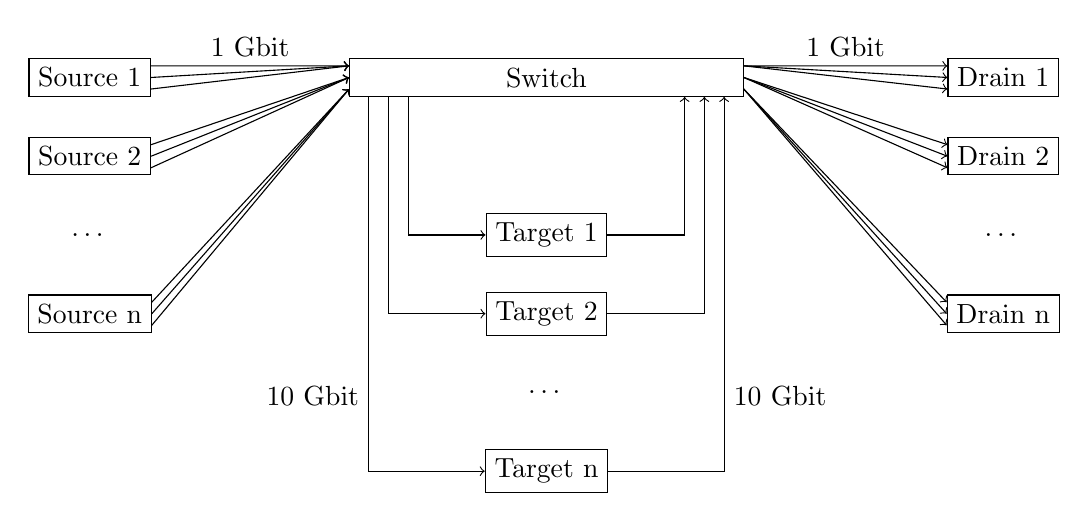
\begin{tikzpicture}
    \path (-5.8, 0) node [draw] (s1) {Source 1};
    \path (-5.8,-1) node [draw] (s2) {Source 2};
    \path (-5.8,-2) node             {\dots};
    \path (-5.8,-3) node [draw] (s3) {Source n};
    \path (s1.north east) -- (s1.south east)
     node (s11) [pos=0.2] {} node (s12) [pos=0.5] {} node (s13) [pos=0.8] {};
    \path (s2.north east) -- (s2.south east)
     node (s21) [pos=0.2] {} node (s22) [pos=0.5] {} node (s23) [pos=0.8] {};
    \path (s3.north east) -- (s3.south east)
     node (s31) [pos=0.2] {} node (s32) [pos=0.5] {} node (s33) [pos=0.8] {};

    \path ( 0, 0) node [draw,minimum width=5cm] (s)  {Switch};
    \path (s.north west) -- (s.south west)
     node (sw1) [pos=0.2] {} node (sw2) [pos=0.5] {} node (sw3) [pos=0.8] {};
    \path (s.north east) -- (s.south east)
     node (se1) [pos=0.2] {} node (se2) [pos=0.5] {} node (se3) [pos=0.8] {};

    \path ( 5.8, 0) node [draw] (d1) {Drain 1};
    \path ( 5.8,-1) node [draw] (d2) {Drain 2};
    \path ( 5.8,-2) node             {\dots};
    \path ( 5.8,-3) node [draw] (d3) {Drain n};
    \path (d1.north west) -- (d1.south west)
     node (d11) [pos=0.2] {} node (d12) [pos=0.5] {} node (d13) [pos=0.8] {};
    \path (d2.north west) -- (d2.south west)
     node (d21) [pos=0.2] {} node (d22) [pos=0.5] {} node (d23) [pos=0.8] {};
    \path (d3.north west) -- (d3.south west)
     node (d31) [pos=0.2] {} node (d32) [pos=0.5] {} node (d33) [pos=0.8] {};

    \draw [->] (s11.center) -- (sw1.center) node [pos=.5,above] {1 Gbit};
    \draw [->] (s12.center) -- (sw1.center);
    \draw [->] (s13.center) -- (sw1.center);
    \draw [->] (s21.center) -- (sw2.center);
    \draw [->] (s22.center) -- (sw2.center);
    \draw [->] (s23.center) -- (sw2.center);
    \draw [->] (s31.center) -- (sw3.center);
    \draw [->] (s32.center) -- (sw3.center);
    \draw [->] (s33.center) -- (sw3.center);

    \draw [<-] (d11.center) -- (se1.center) node [pos=.5,above] {1 Gbit};
    \draw [<-] (d12.center) -- (se1.center);
    \draw [<-] (d13.center) -- (se1.center);
    \draw [<-] (d21.center) -- (se2.center);
    \draw [<-] (d22.center) -- (se2.center);
    \draw [<-] (d23.center) -- (se2.center);
    \draw [<-] (d31.center) -- (se3.center);
    \draw [<-] (d32.center) -- (se3.center);
    \draw [<-] (d33.center) -- (se3.center);

    \path (0,-2) node [draw] (t1) {Target 1};
    \path (0,-3) node [draw] (t2) {Target 2};
    \path (0,-4) node             {\dots};
    \path (0,-5) node [draw] (t3) {Target n};
    \path (s.south) -- (s.south west)
     node (ssw1) [pos=.7] {} node (ssw2) [pos=.8] {} node (ssw3) [pos=.9] {};
    \draw [->] (ssw1.center) |- (t1.west);
    \draw [->] (ssw2.center) |- (t2.west);
    \draw [->] (ssw3.center) |- (t3.west) node [pos=.4,left]{10 Gbit};
    \path (s.south) -- (s.south east)
     node (sse1) [pos=.7] {} node (sse2) [pos=.8] {} node (sse3) [pos=.9] {};
    \draw [<-] (sse1.center) |- (t1.east);
    \draw [<-] (sse2.center) |- (t2.east);
    \draw [<-] (sse3.center) |- (t3.east) node [pos=.4,right]{10 Gbit};
\end{tikzpicture}
\end{frame}

\subsection{Performance Hardware Design}
\begin{frame}{Performance Hardware Design}
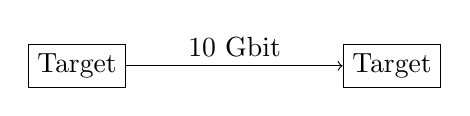
\begin{tikzpicture}
    \path (  0,   0) node [draw] (local) {Target};
    \path (  4,   0) node [draw] (remote) {Target};
    \draw [->] (local) -- (remote) node [midway,above] {10 Gbit};
\end{tikzpicture}
\end{frame}

\section{How does it work?}

\begin{frame}{Agenda}
\setcounter{tocdepth}{1}
\tableofcontents[currentsection]
\end{frame}

\subsection{Performance Goals}
\begin{frame}{Performance Goals}
\begin{itemize}
    \item history
    \item reproducable
    \item details available
    \item drill down
    \item automatic
\end{itemize}
\end{frame}

\subsection{Performance History}
\begin{frame}{Performance History}
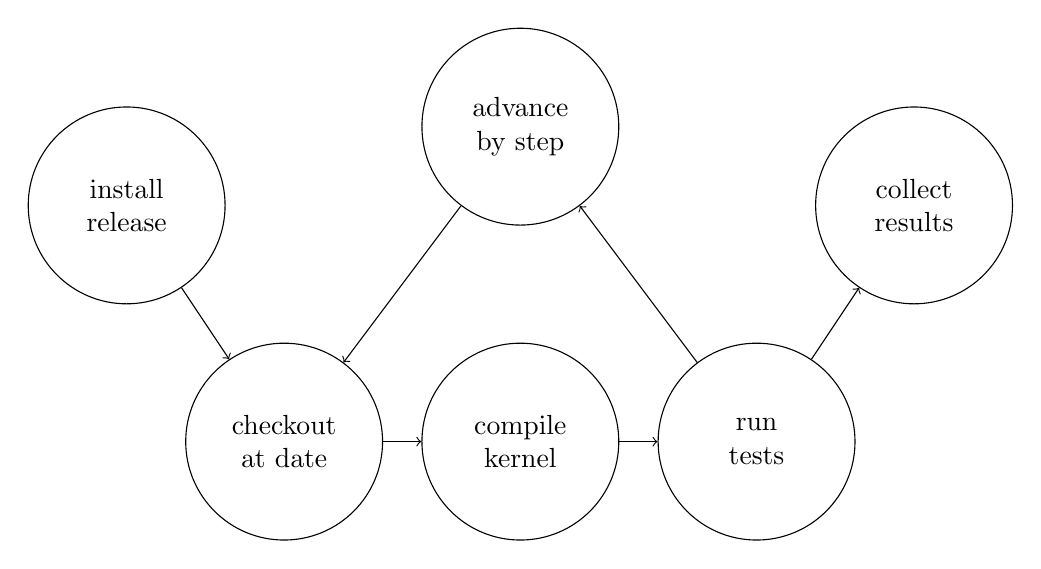
\begin{tikzpicture}
    \path ( 1, 1) node [draw,circle,align=center,minimum width=2.5cm]
	(release) {install\\release};
    \path ( 3,-2) node [draw,circle,align=center,minimum width=2.5cm]
	(checkout) {checkout\\at date};
    \path ( 6,-2) node [draw,circle,align=center,minimum width=2.5cm]
	(kernel) {compile\\kernel};
    \path ( 9,-2) node [draw,circle,align=center,minimum width=2.5cm]
	(test) {run\\tests};
    \path ( 6, 2) node [draw,circle,align=center,minimum width=2.5cm]
	(step) {advance\\by step};
    \path (11, 1) node [draw,circle,align=center,minimum width=2.5cm]
	(result) {collect\\results};
    \draw [->] (release) -- (checkout);
    \draw [->] (checkout) -- (kernel);
    \draw [->] (kernel) -- (test);
    \draw [->] (test) -- (result);
    \draw [->] (test) -- (step);
    \draw [->] (step) -- (checkout);
\end{tikzpicture}
\end{frame}

\subsection{Performance Hardware}
\begin{frame}{Performance Hardware}
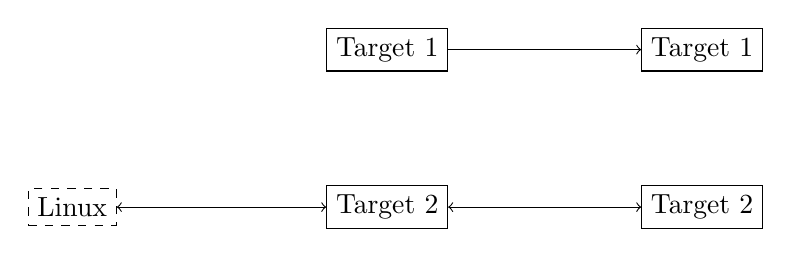
\begin{tikzpicture}
    \path (  0,   0) node [draw] (local1) {Target 1};
    \path (  4,   0) node [draw] (remote1) {Target 1};
    \draw [->] (local1) -- (remote1);
    \path (  0,  -2) node [draw] (local2) {Target 2};
    \path (  4,  -2) node [draw] (remote2) {Target 2};
    \draw [<->] (local2) -- (remote2);
    \path ( -4,  -2) node [draw,dashed] (linux) {Linux};
    \draw [<->] (linux) -- (local2);
\end{tikzpicture}
\end{frame}

\subsection{Performance Master}
\begin{frame}{Performance Master}
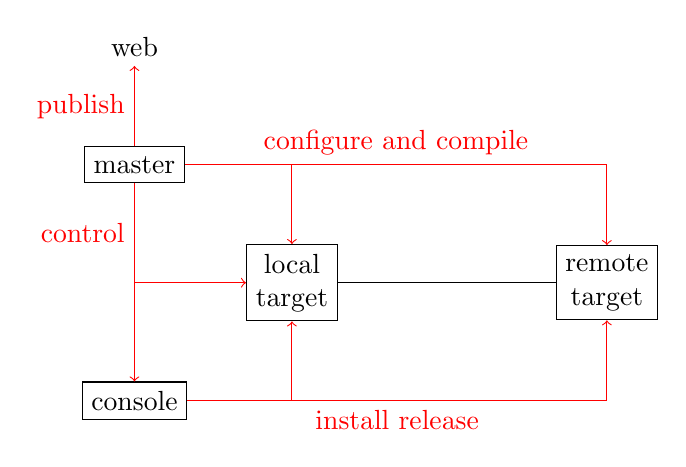
\begin{tikzpicture}
    \path ( -2,   3) node (web) {web};
    \path ( -2, 1.5) node [draw] (master) {master};
    \path ( -2,-1.5) node [draw] (console) {console};
    \path (  0,   0) node [draw,align=center] (local) {local\\target};
    \path (  4,   0) node [draw,align=center] (remote) {remote\\target};
    \draw (local) -- (remote);
    \draw [->,red] (master) -- (web) node [midway,left] {publish};
    \draw [->,red] (master) -- (console);
    \draw [->,red] (master) |- (local) node [near start,left] {control};
    \draw [->,red] (master) -| (local);
    \draw [->,red] (master) -| (remote)
	node [near start,above] {configure and compile};
    \draw [->,red] (console) -| (local);
    \draw [->,red] (console) -| (remote)
	node [near start,below] {install release};
\end{tikzpicture}
\end{frame}

\section{What are the findings?}

\begin{frame}{Agenda}
\setcounter{tocdepth}{1}
\tableofcontents[currentsection]
\end{frame}

\subsection{Reproduce and Reboot}
\begin{frame}{Reproduce and Reboot}
\begin{tikzpicture}
    \path ( 6,-2) node [draw,circle,align=center,minimum width=2.5cm]
	(kernel) {compile\\kernel};
    \path ( 9,-2) node [draw,circle,align=center,minimum width=2.5cm]
	(test) {run\\tests};
    \path (11,-4) node [draw,circle,align=center,minimum width=2.5cm]
	(keep) {run\\again};
    \path (14,-4) node [draw,circle,align=center,minimum width=2.5cm]
	(reboot) {reboot\\machine};
    \path (17,-4) node [draw,circle,align=center,minimum width=2.5cm]
	(reorder) {relink\\kernel};
    \draw [->] (checkout.east) -- (kernel);
    \draw [->] (kernel) -- (test);
    \draw [->] (test) -- (result);
    \draw [->] (test) -- (step);
    \draw [->] (test) -| (keep);
    \draw [->] (test) -| (reboot);
    \draw [->] (test) -| (reorder);
    \draw [->] (reorder) -- (reboot);
    \draw [->] (reboot) -- (keep);
    \draw [->] (keep) -| (test);
\end{tikzpicture}
\end{frame}

\subsection{Future Ideas}
\begin{frame}{Future Ideas}
\begin{itemize}
    \item forwarding throughput
    \item Linux client and server
    \item testing patches
    \item historic releases
    \item file system performance
\end{itemize}
\end{frame}

\subsection{Thanks}
\begin{frame}{Thanks}
\begin{itemize}
    \item Jan Klemkow for Hardware Administration
    \item Moritz Buhl for Visualization
    \item genua for Hosting and Worktime
\end{itemize}
\end{frame}

\subsection{Links}
\begin{frame}{Links}
\begin{itemize}
    \small
    \item \url{http://bluhm.genua.de/}
    \item \url{http://bluhm.genua.de/regress/results/regress.html}
    \item \url{http://bluhm.genua.de/perform/results/perform.html}
    \item \url{http://bluhm.genua.de/perform/results/gnuplot/test.data}
    \item \url{https://github.com/bluhm/regress-all}
    \item \url{https://github.com/bluhm/udpbench}
    \item \url{https://github.com/younix/testmaster}
    \item \url{https://github.com/bluhm/talk-perform}
\end{itemize}
\end{frame}

\subsection{Questions}
\begin{frame}{Questions}
\begin{center}
?
\end{center}
\end{frame}

\end{document}
